\documentclass[11pt]{article}
% \usepackage[utf-8]{inputenc}
\usepackage[margin=1in]{geometry}
\usepackage{listings}
\usepackage{xcolor}
\usepackage{graphicx}
\usepackage{hyperref}
\usepackage{amsmath}
\usepackage{amssymb}
\usepackage{booktabs}
\setlength{\textfloatsep}{8pt}
\setlength{\floatsep}{6pt}
\setlength{\intextsep}{6pt}

% Configure listings style
\lstset{
    language=Python,
    basicstyle=\ttfamily\small,
    keywordstyle=\color{blue},
    commentstyle=\color{gray},
    stringstyle=\color{red},
    breaklines=true,
    breakatwhitespace=true,
    showstringspaces=false,
    tabsize=4,
    backgroundcolor=\color{gray!10},
    frame=single,
    linewidth=0.95\textwidth
}

\title{Homework: Page Replacement Algorithms}
\author{Haotang Li}
\date{}

\begin{document}

\maketitle

\section{Implementation}
\subsection{LRU}
I implemented LRU using a single \texttt{OrderedDict} as an ordered set.
On a hit, the referenced page is moved to the tail (MRU). On a fault, if memory is full,
the head entry (LRU) is evicted before inserting the new page at the tail.
This design keeps each access at \(O(1)\) time and uses \(O(\text{capacity})\) space.

\subsection{Two-List (Active/Inactive)}
I implemented TwoList with two \texttt{OrderedDict}s (inactive/active) and a location map.
New pages first enter the \textbf{inactive} list; a second reference promotes the page to
\textbf{active}. Eviction is taken from the inactive head, while active overflow is handled
by demoting the oldest active page back to inactive.
All operations remain \(O(1)\), with total memory \(O(\text{capacity})\).

\section{Testing}

\subsection{Test Environment}

\begin{itemize}
    \item \textbf{Platform}: macOS
    \item \textbf{Python}: 3.12+
    \item \textbf{Test harness}: \texttt{testcases.json} with 9 predefined cases
\end{itemize}

To reproduce results, run: \texttt{python page\_replacement.py --test ../testcases.json}.

\subsection{Results Summary}

Predefined suite: \textbf{27/27 checks passed}.  
Additional custom suite: \textbf{9/9 checks passed}.

Beyond predefined cases, three custom workloads were added to test edge cases:
(1) pure sequential scan (no reuse, all policies fault equally),
(2) persistent hot page with transient disturbance (TwoList protection helps),
(3) promotion/demotion overhead (TwoList occasionally miscategorizes).

\textbf{Key observations}:
\begin{itemize}
    \item \texttt{lru\_beats\_fifo}: FIFO=8, LRU=6, TwoList=6, confirming the benefit of recency-aware replacement.
    \item \texttt{repeated\_scan\_resistance}: FIFO=40, LRU=40, TwoList=28, showing strong scan resistance from active/inactive separation.
    \item \texttt{twolist\_approximation\_cost}: FIFO=4, LRU=4, TwoList=5, illustrating that heuristic promotion/demotion can occasionally hurt.
    \item \texttt{twolist\_beats\_lru\_custom}: FIFO=5, LRU=5, TwoList=4, showing a case where active-list protection outperforms plain LRU.
\end{itemize}

\begin{figure}[htbp]
\centering
\includegraphics[width=0.48\textwidth]{testcases.png}
\hfill
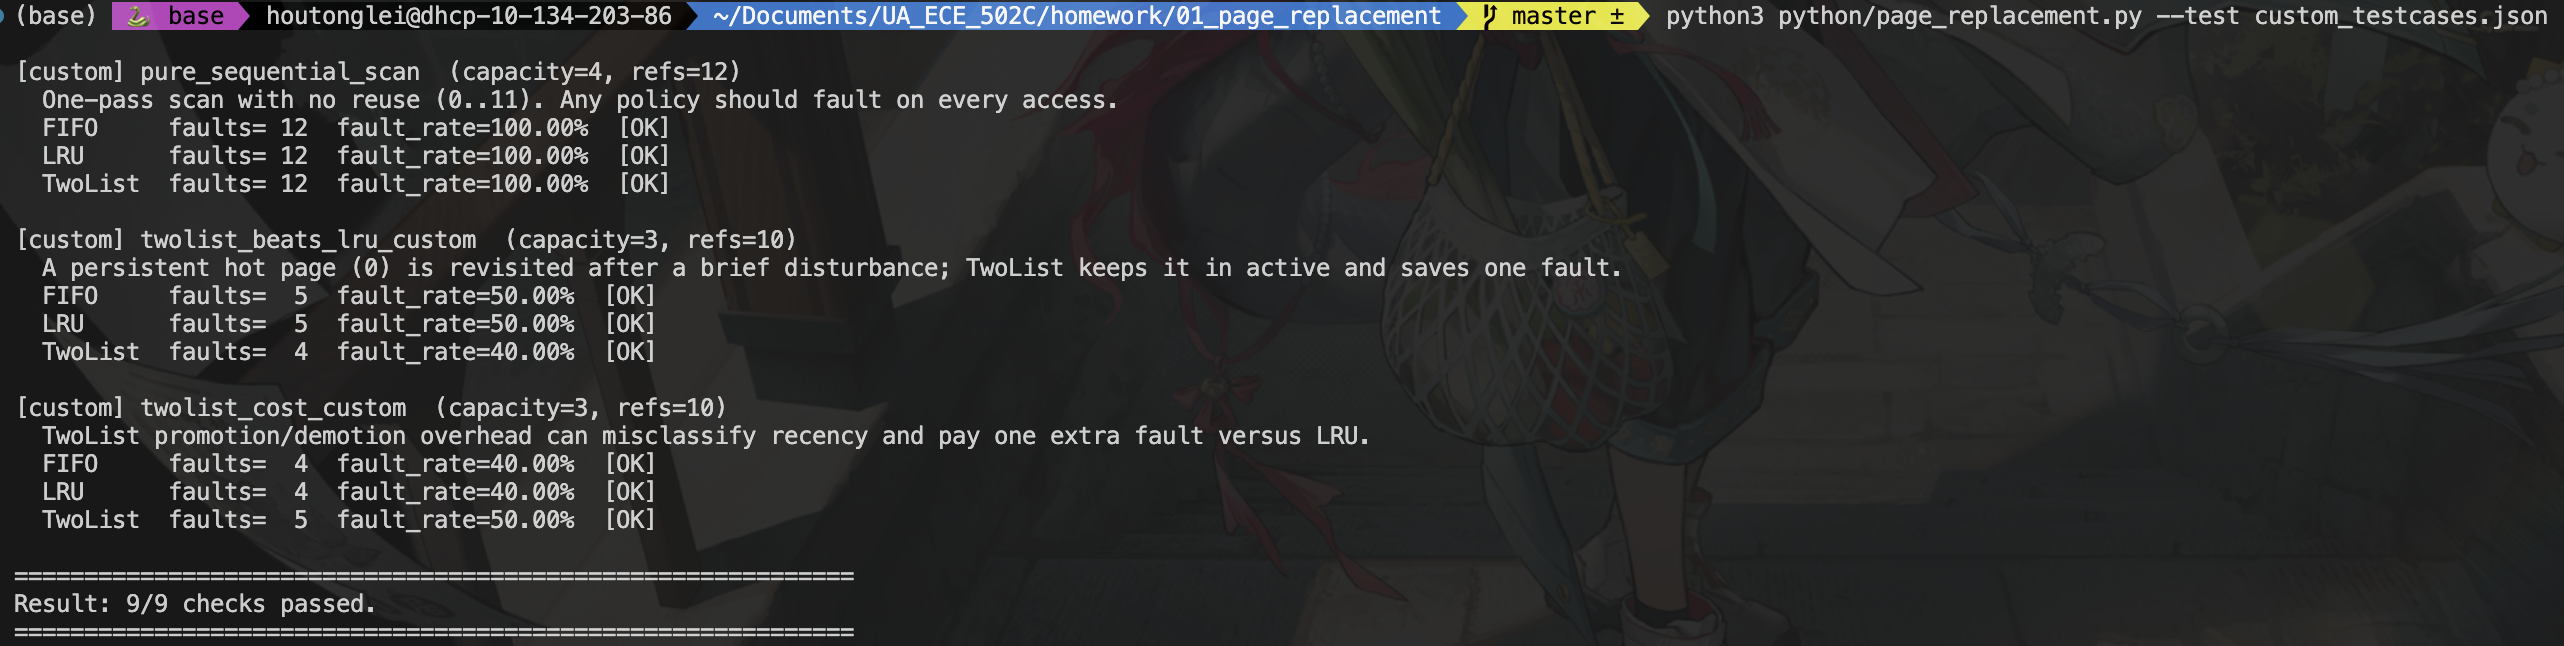
\includegraphics[width=0.48\textwidth]{custom_testcases.png}
\caption{Console outputs for predefined test suite (left) and custom test suite (right).}
\end{figure}

\section{Discussion}

\textbf{Key Insights}: Temporal locality is the dominant factor in typical workloads (Q1);\,\, two-list schemes trade simplicity for robustness against scans (Q4); and within sufficient memory, policy differences shrink (Q5).

\begin{enumerate}
    \item \textbf{Q1 (LRU vs FIFO)}: FIFO follows arrival order and may evict pages that will be reused soon. LRU tracks recent use and therefore keeps those pages, reducing faults from 8 to 6.
    \item \textbf{Q2 (TwoList extra cost)}: With a tight active/inactive split, promotion can trigger early demotion of a still-useful active page, producing one extra fault (TwoList 5 vs LRU 4).
    \item \textbf{Q3 (Belady)}: FIFO is not stack-based, so increasing frames can worsen its eviction order (9 \(\rightarrow\) 10). LRU and TwoList remain recency-aware in this workload and improve (10 \(\rightarrow\) 8).
    \item \textbf{Q4 (Scan resistance)}: TwoList preserves hot pages in active while one-time scan pages churn in inactive, reducing faults from 40 to 28. If active capacity is 0, this protection vanishes.
    \item \textbf{Q5 (Convergence)}: In gradual working-set shifts with sufficient capacity, all policies converge (9 faults). Under abrupt shifts or intermittent hot pages, FIFO can diverge from LRU/TwoList.
\end{enumerate}

\section{Conclusion}
This implementation correctly realizes both LRU and TwoList algorithms and passes all 36 test checks (27 predefined \(+\) 9 custom).
The results demonstrate that LRU is a strong general-purpose replacement policy for temporal-locality workloads,\, while TwoList adds measurable scan resistance (28 vs 40 faults) by maintaining an active/inactive partition.\, The trade-off is a slightly higher error rate when the hot/cold split misaligns.\, These findings align with the Linux kernel's adoption of similar two-list strategies in practice.

\end{document}
